%!TEX root = cscw2019-comic.tex
\section{Method}
\label{sec:Method}
In this study on Amazon Mechanical Turk, we examine if the abstract comic can impcat a decision wiht monetary consequence. The persuasion goal is to ask participants to make more charitable donation with the real money. 
%In this study, we examine if the abstract comic can impact a decision with monetary consequence. The aim of this study is to show the persuasiveness of the abstract comic in the real-life setting.  
%In contrast, the first study demonstrated that participants prefer messages in abstract comic form over text, but did not demonstrate persuasiveness.
% as more persuasive, it is unknown if the perceived persuasiveness can impact people's real-life decision making. So, we further studied the ability of abstract comics in persuading people to make decisions in the real life. 
% In the second study, we conduct a field study on Amazon Mechanical Turk and compared the power between pure text messages and abstract comic messages in persuading people to donate with their real money. 
In this section, we will introduce the experiment design and describe our study participants recruiting process.




\subsection{Experiment Design}
Since the main goal for this study is to compare power of a persuasive message on behaviors in two forms, the abstract comic and the pure text, we first constructed two experimental conditions, abstract-comic (see~\Cref{fig:basic three comic panel}) and pure-text. In the abstract-comic condition, participants will read a message asking if they are willing to support a charity in a three-panel abstract comic strip, whereas in the pure-text condition, participants will receive the same message in pure text form. To test idea of social proof, we then added a third condition, a three-panel comic that includes the normative behavior (see~\Cref{fig:basic three comic social proof}).
% Additionally, we are also interested in if the abstract comic can leverage persuasive techniques to increase its persuasiveness. Hence, we incorporated the idea of social proof and created the third condition, social-proof-comic.

\begin{figure}[bt]
	\centering
	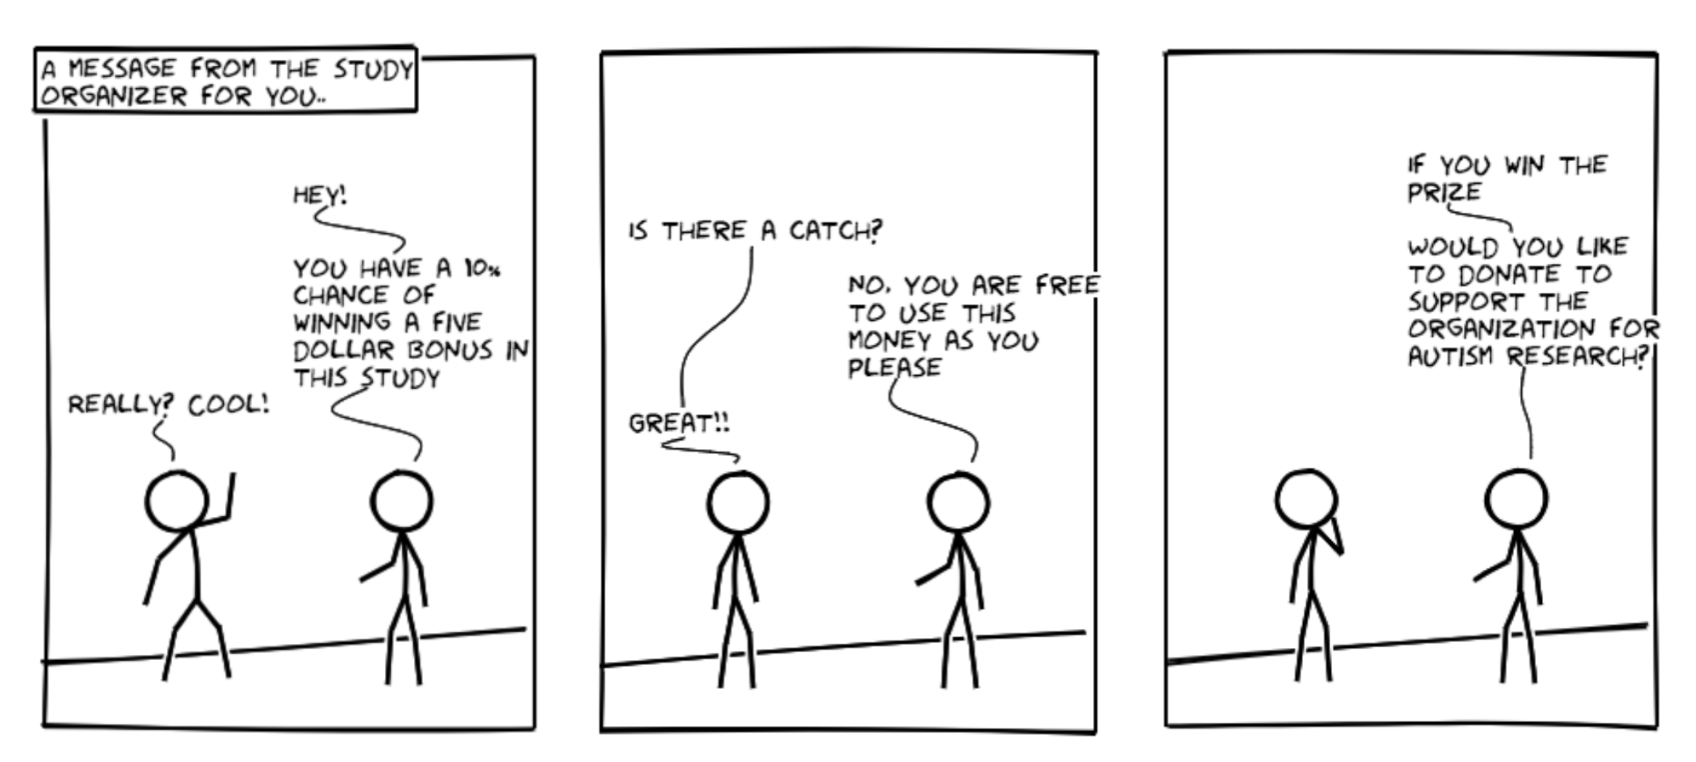
\includegraphics[width=\columnwidth]{./figures/abstract_comic.png}
	\caption{Messages in the abstract comic form}
	\label{fig:basic three comic panel}
\end{figure}

The objectives of the persuasive message in all three conditions: persuading participants to donate to a charity from his/her own pocket. Similiar to \textcite{lee2013does}, the money partcipants will use is part of their study compensation, a prospective bonus reward (10\% chance of winning \$5 bonus). We randomly assigned study participants to one of the three conditions; the participants are free to make a decision on the amount of donation, including not donating at all.

\paragraph{Study Procedure} Once a participant consents to join the study, we ask them if they are  familiar with the Autism Spectrum Disorder (ASD). Then, each participant watches a short-video produced by the Organization for Autism Research that promotes its fundraising activity "RUN FOR AUTISM". After watching the video, we ask participants to summarize the video using free text and ask them to provide their opinion about the effectiveness of the video. The recruiting message specifically mentions this task of soliciting their opinion on the message effectiveness.

We randomly assign participants to each of the three conditions and and then ask them to read the corresponding persuasive message (text, three-panel comic, three-panel comic with social proof). In the message, we provide the participant with a 10\% chance of winning \$5 additional compensation. We also provide them with the opportunity to donate to the Organization for Autism Research (OAR) which is the charity mentioned in the video they watch as part of the study.

To best demonstrate the persuasiveness of the message itself, we diffused the responsibility of donation amount among all participants. Similar to ~\textcite{lee2013does}, before the participants make their decision, they read "The total amount of money allocated to [the charity] by all the winning participants will be aggregated and donated at the end of the study." Then, we ask the participants to decide the amount of money they are willing to donate on a slider bar with \$0 and \$5 as two extreme ends. The default position of the slider bar is at the \$0 end.

Before leaving the study, the participants we ask the participants to fill a demographic questionnaire about their gender, age and education; the participants have the option of declining to state an answer for each question.

At the end of the study, we randomly chose 10\% of the participants, donated to OAR based on the participants decision, and rewarded each chosen participant the part of the bonus that they wished to keep.

To gather the basic statistics to create social proof, we first ran a pilot study with the first two conditions ($n=60$) and used the donation statistics as part of the social proof message. In the pilot study, 87\% of the participants donated a non-zero amount. 

% i.e.  X \% of participants donated in our study and validate the study procedure, we first ran a pilot study with two conditions, abstract-comic and pure-text before the actual experiment fielded.


\begin{figure}[bt]
	\centering
	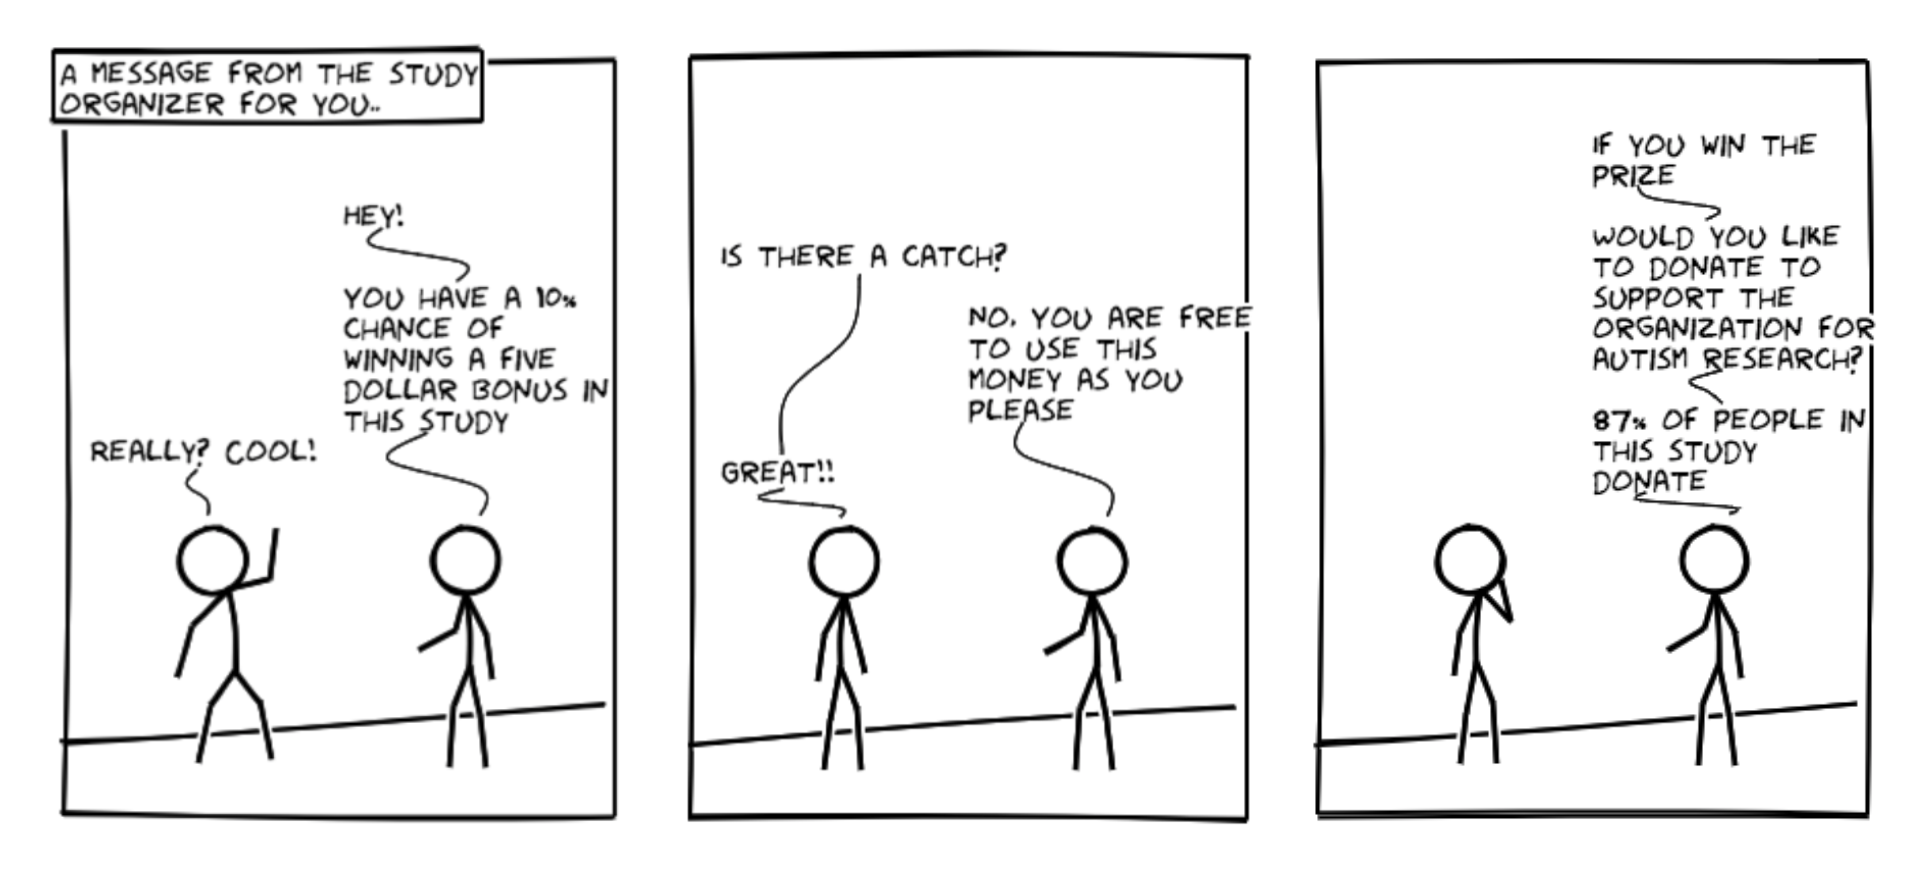
\includegraphics[width=\columnwidth]{./figures/social_proof.png}
	\caption{Messages with social proof.}
	\label{fig:basic three comic social proof}
\end{figure}

\paragraph{Organization for Autism Research (OAR)}
To increase the realism of our study, the donation decision is not hypothetical and participants are rewarded based on their decision and we as study organizers donate to the Organization for Autism Research (OAR). We chose OAR as the charity in our study for three reasons. First, Autism Spectrum Disorder (ASD), is a well-known, serious developmental disorder that impairs the communication and behavior. In other words, ASD provides basic interest for the participants to support the related charitable organization. Second, the Organization for Autism Research is one of the most visible ASD related organizations that helps individuals with autism and provides assistance to parents, families, teachers and caregivers. The goal of OAR is clear and reputable so participants won't question the authenticity of our message's motive. Finally, we wished to avoid a charity associated with a life-threatening condition such as cancer as it may create an experimental confound: we don't know if some donates because their intrinsic desire to help with a life-threatening condition. While ASD can have serious consequences on the well being of those who have it, the public perception is that ASD is not-life threatening. 

\paragraph{Persuasive Messages}

The persuasive messages communicate three major objectives, 1) Participants will have 10 \% of chance winning \$ 5 bonus upon the completion of the study. 2) Participants are free to use the money as they please. and 3) Participants can donate this bonus to the Organization for Autism Research (OAR). Therefore, in the text condition, study participants will read the following message,
\begin{quote}
  \textit{You have a 10\% chance of winning a five dollar bonus in this study. You are free to use this money as you please. If you win the prize, would you like to donate to support the Organization for Autism Research?}
\end{quote}
In the two comic conditions, we created three-panel comic strips to communicate the message. The three-panel comic strip allows us to leverage one of the most fascinating aspect of comics---storytelling~\cite{scott1993understanding}. 
%Since the first study did not show a convincing effect for framing, participant gesture, character distance and shading, we did not vary those conditions in this experiment. We set the inter-character distance to be medium, light background. 
Consistent with ``match on action'' technique~\cite{scott1993understanding}, we matched the panels on the gesture of the first character (the message recipient), while retaining a neutral gesture for the second character (who delivers the message). We create the comic strip in a manner similar to the first study on preference.

% Each of the three panel communicates one major objective in the message. The comic strip is created in the similar fashion as in the first study on preference. As we learned from the first study that appropriate gestures will maximize the persuasiveness of the comics, we then chose the gesture that we believe best suit for the scenario see~\Cref{fig:basic three comic panel}.

In the social-proof-comic condition, we created social-proof by adding one sentence on the last comic panel indicates the percentage of people in our study donated see~\Cref{fig:basic three comic social proof}. The percentage (87\%) corresponds to the number of people who donated a non-zero amount in the pilot study.

% \begin{figure*}
%  \subfloat[Messages in the abstract comic form]{%
%   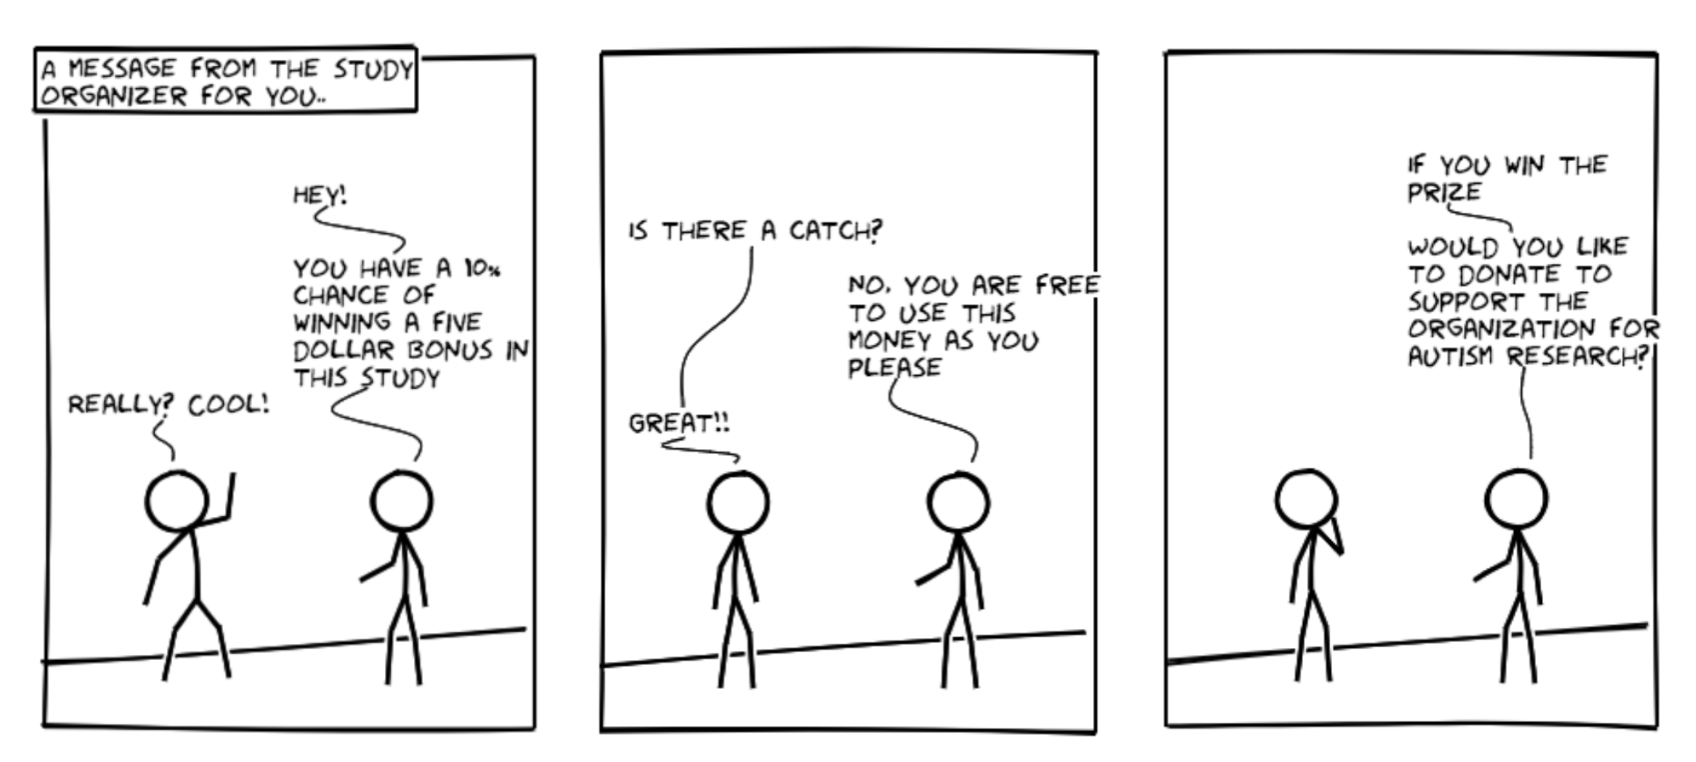
\includegraphics[width=0.5\textwidth]{./figures/abstract_comic.png}
%   } \hfill
%  \subfloat[Messages in the abstract comic form with social proof]{%
%   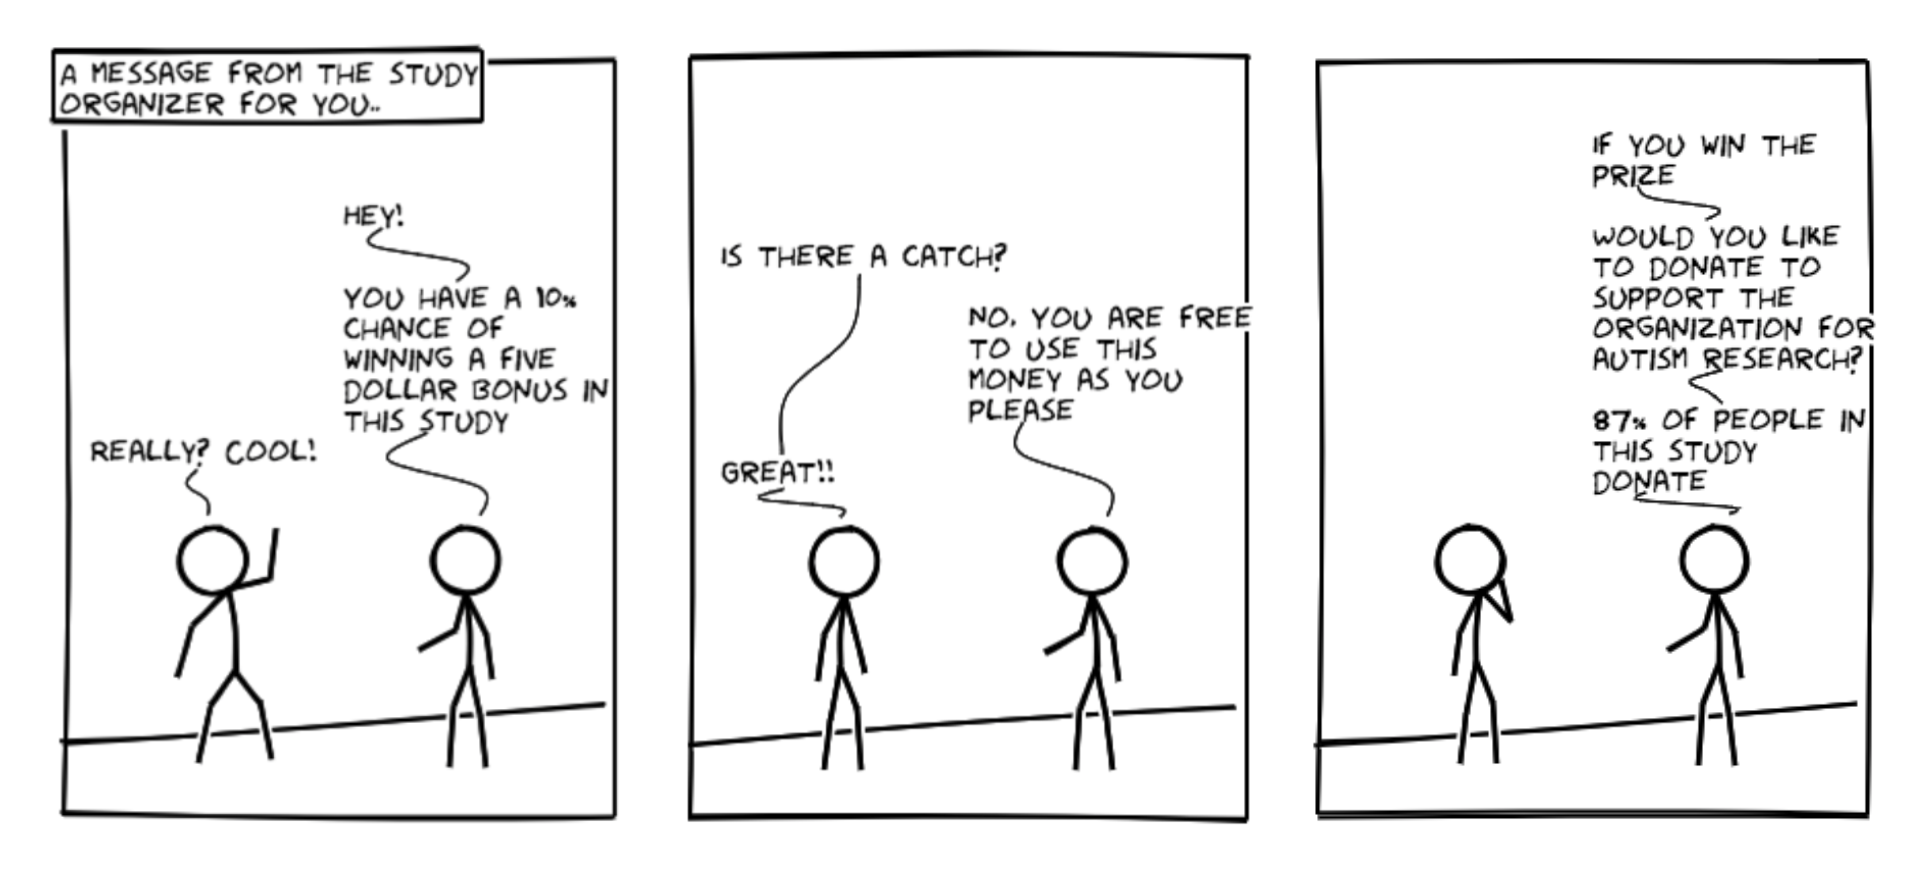
\includegraphics[width=0.5\textwidth]{./figures/social_proof.png}
%  }
%  \caption{The messages participants received in two abstract-comic conditions}
%  \label{fig:comic_messages_in_two_conditions}
% \end{figure*}

\subsubsection{Participants}
We published our HITs on Amazon Mechanical Turk titled ``A short survey about communicating autism campaign ads.'' Similar to the Study 1, the compensation was \$8/hr, and the workers would get these rewards regardless of their performance, the threshold for participant to join was a 95\% Approval Rate. On the HIT page, we instructed that repeated responses would be rejected. We told the participants that they would see a link to our experiment site.
